\section{Concepts, relationships and the network}
The whole idea revolves around the idea of concepts, 
their relationships and the network structure 
that arises.

\begin{figure}[ht]
 \begin{center}
    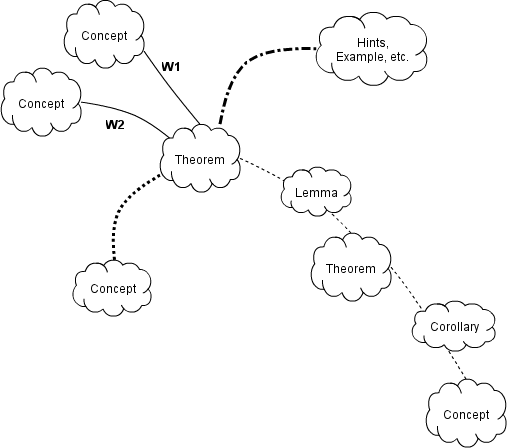
\includegraphics[width=4in]{../img/knet_general.png}
 \end{center}
    \caption{Network of concepts.}
    \label{fig:network_concepts}
\end{figure}



\section{Tech Specs}

\subsection{Social network}
The idea is to build kind of a social network in which
the objective is to advance the understanding and the
organization of math concepts.

\subsection{Re-use not re-invent}
Todays social networks provide most of what would be
needed to implement Knetledge.

Some of the requiered specs are:

\begin{itemize}
 \item Video chat
 \item Voice chat
 \item Shared spaces. Blackboard for brainstorming
 \item Simultaneus edit capabilities
 \item Local copies of subsets of the network
 \item User profile tracking
 \item User profile preferences
 \item Currently working on
 \item Topic: contributors, etc
 
\end{itemize}


\subsection{Graph databases}
There's a lot to learn about Graph databases but it
seems like they would be ideal to implement the kind
of schema that would result from organizing knowledge.

Have to investigate more on the associative data model.
Basically it says that nodes are stored in one table
while relationships between nodes are stored in another 
table which contains information about source and target 
node, and the type of relationships between the connected
nodes.

\subsection{User profile}
\begin{itemize}
 \item Level of Abstraction. This is the level at which 
 the user usually likes to browse concepts.
 \item Areas of interest.
 \item List of known concepts.
 \item Contributions
\end{itemize}

\subsection{Workspace}
A workspace is a set of worksheets, each one containing
a \textbf{board} in which the user can edit a subset of the 
network locally (offline) using a set of tools.

The subset can be then send to a set of experts to 
be reviewed and after that it can be accepted as part of the 
network that is publicly available to everyone.

Of course each person can choose who they share their personal
work with, just like you can set visibility parameter to 
your post on almost any social network.

\section{The Board}
Some of the actions a users can do while in the board are:
\begin{itemize}
 \item Create a new or add an existing concept to the board.
 \item Remove a node
 \item Create a new relationship or add an existing one
 \item Discover relationships. Shows you a list of existing 
relationships so that the user can choose which one are interesing
for the particular aspect s/he is going to work on
\item Save/load the state of the board. Kind of like version control.
The interface should provide tools for easy comparison between different
versions of the board.
 
\end{itemize}


\section{Typical session}
After logging in the user can access the information in the network
by the two most common method, browse and search.

\subsection{Browse}
There should be categories that can be universal or created
by the user, like filter searches

\subsection{Search}
Should include the most common filters:
\begin{itemize}
 \item Topic/related concepts
 \item Contributors
 \item Abstraction levels
 \item Content type: multimedia, text, etc.
\end{itemize}

Other features
\begin{itemize}
 \item Watch later like youtube
 \item Add to board
\end{itemize}



\section{Peer review}

The network should provide the tools for making it easy
to asses the validity of a subset of the network submitted
for revision.

\section{Colaboration}
It should allow simultaneous collaboration in real-time something
similar to what google wave was.



\section{Algorithms}
\begin{itemize}
 \item Find relationships
 \item Propose relationships/applications. This can be used
 to generalize concepts thought to be unrelated
 \item Create new nodes
 \item Automated proof
\end{itemize}


\section{Publishing}
It should provide tools for comparing, merging subsets of the
network in order to facilitate the addition of new concepts
to the network.